% Feel free to contact me for any reason:
%% Email 1: zain.kamal@rutgers.edu
%% Email 2: z.kamal2021@gmail.com
%% Discord: alci#6038

%%%%%%%%%%%%%%%%%%%%%%%%%%%%%%%%%%%%%%%%%%%%%%%%%%%%%%%%%%%%%%%%%%%%%%%%%%%%%%%%%
\documentclass{article}
% Feel free to contact me for any reason:
%% Email 1: zain.kamal@rutgers.edu
%% Email 2: z.kamal2021@gmail.com
%% Discord: alci#6038

% Last updated 1/28/22

% Template based off of Justin Kim's (don't know where he got it from originally), but I've made a ton of edits. His soul lives on in random packages and commands I'm too lazy to comment out.


%%%%%%%%%%%%%%%%%%%%%%%%%%%%%%%%%%%%%%%%%%%%%%%%%%%%%%%%%%%%%%%%%%%%%%%%%%%%%%%%%%%%
%%% Default packages:

\usepackage[margin=1in]{geometry} 
\usepackage{amsmath,amsthm,amssymb,amsfonts, fancyhdr, color, comment, graphicx, environ}
\usepackage{xcolor}
\usepackage{mdframed}
\usepackage{bm}
\usepackage[shortlabels]{enumitem}
\usepackage{mathtools}
\usepackage{listings}
\usepackage{stmaryrd}
\usepackage{indentfirst}
\usepackage{hyperref}


%%%%%%%%%%%%%%%%%%%%%%%%%%%%%%%%%%%%%%%%%
%%% Pacakages I've added:

%% For Math 300 (Winter 2021):

\usepackage{mathdots} % for \iddots

\usepackage[ruled]{algorithm2e} % Algorithms
% NOTE: FIND A BETTER ALGORITHM PACKAGE, OR ATLEAST LEARN HOW TO USE THIS ONE BECAUSE DOUBLE INDENTING IS A FUCKING NIGHTMARE (or just import from mathcha?)
%% Example algorithm:
% \begin{center}
% 	\begin{minipage}{0.5\linewidth} % Adjust the minipage width to accomodate for the length of algorithm lines
% 		\begin{algorithm}[H]
% 			\KwIn{$(a, b)$, two floating-point numbers}  % Algorithm inputs
% 			\KwResult{$(c, d)$, such that $a+b = c + d$} % Algorithm outputs/results
% 			\medskip
% 			\If{$\vert b\vert > \vert a\vert$}{
% 				exchange $a$ and $b$ \;
% 			}
% 			$c \leftarrow a + b$ \;
% 			$z \leftarrow c - a$ \;
% 			$d \leftarrow b - z$ \;
% 			{\bf return} $(c,d)$ \;
% 			\caption{\texttt{FastTwoSum}} % Algorithm name
% 			\label{alg:fastTwoSum}   % optional label to refer to
% 		\end{algorithm}
% 	\end{minipage}
% \end{center}



%%%%%%%%%%%%%%%%%%%%%%%%%%%%%%%%%%%%%%%%%%%%%%%%%%%%%%%%%%%%%%%%%%%%%%%%%%%%%%%%%%%%
%%% Default commands:

\renewcommand{\vec}[1]{\mathbf{#1}}
	
\newcommand{\WidestEntry}{$lon_1$}%
\newcommand{\SetToWidest}[1]{\makebox[\widthof{\WidestEntry}]{#1}}%
\newcommand\tab[1][0.61cm]{\hspace*{#1}}
\newcommand{\nats}{\mathbb{N}}
\newcommand{\rats}{\mathbb{Q}}
\newcommand{\reals}{\mathbb{R}}
\newcommand{\Z}[1]{\mathbb{Z}_{#1}}
\newcommand{\BigO}[1]{\mathcal{O}(#1)}
\newcommand{\seq[1]}{(#1_n)}
\newcommand{\subseq[1]}{(#1_{n_k})}
\newcommand{\Lim}[2]{\lim \limits _{#1 \to #2}}
\newcommand{\Min}[2]{\min \{#1, #2\}}
\newcommand{\inv}{^{-1}}
\newcommand{\h}{^\text{th}}
\newcommand{\lrangle}[1]{\langle #1 \rangle}
\newcommand{\abs}[1]{\left\lvert #1 \right\rvert}

\DeclarePairedDelimiter{\ceil}{\lceil}{\rceil}
\DeclarePairedDelimiter{\floor}{\lfloor}{\rfloor}
\DeclareMathOperator{\supp}{supp}
\DeclareMathOperator{\rad}{rad}
\DeclareMathOperator*{\argmin}{arg\,min}
\DeclareMathOperator*{\argmax}{arg\,max}
\DeclareMathOperator*{\Var}{Var}
\DeclareMathOperator*{\Cov}{Cov}
\DeclareMathOperator*{\Corr}{Corr}
\DeclareMathOperator*{\Aut}{Aut}
\newcommand{\prob}[1]{\section*{Problem #1}}


%%%%%%%%%%%%%%%%%%%%%%%%%%%%%%%%%%%%%%%%%
%%% Commands I've added:

%% For Math 300 (Winter 2021):

\newcommand{\lrbrace}[1]{\{ #1 \}}
\newcommand{\powerset}{\mathcal{P}}
\newcommand{\ints}{\mathbb{Z}}

% Source/inspiration: https://tex.stackexchange.com/a/42728:
\newcommand{\numberthis}{\addtocounter{equation}{1}\tag{\theequation}\label{\theequation}}
    % Within an `align*` environment, put `\numberthis` after a line to number it. 
    % Access it with `\eqref{ [number of equation] }`
\newcommand{\numberthiswith}[1]{\addtocounter{equation}{1}\tag{\theequation}\label{#1}}
    % Within an `align*` environment, put `\numberthiswith{ [your_label] }` after a line to number it. 
    % Access it with `\eqref{ [your_label] }`



%%%%%%%%%%%%%%%%%%%%%%%%%%%%%%%%%%%%%%%%%%%%%%%%%%%%%%%%%%%%%%%%%%%%%%%%%%%%%%%%%%%%
%%% Default formatting:

\hypersetup{
    colorlinks=true,
    linkcolor=blue,
    filecolor=magenta,      
    urlcolor=blue,
}

\setlength{\parindent}{0cm}
\setlength{\parskip}{6pt}

\pagestyle{fancy}


%% Misc formatting additions

% make bullets with itemize much smaller
\newlength{\mylen}
\setbox1=\hbox{$\bullet$}\setbox2=\hbox{\tiny$\bullet$}
\setlength{\mylen}{\dimexpr0.5\ht1-0.5\ht2}
\renewcommand\labelitemi{\raisebox{\mylen}{\tiny$\bullet$}}


% Modified version of problem environment below
% \newenvironment{problem}[2][Problem]
%     { \begin{mdframed}[backgroundcolor=gray!5] \textbf{#1 #2} \\}
%     {  \end{mdframed}}
% \newenvironment{solution}{\textbf{Solution}\\}


%%%%%%%%%%%%%%%%%%%%%%%%%%%%%%%%%%%%%%%%%
%%% Formatting I've added:

%% Grey boxes for problem statements (note that I don't have a "solution" section):

% Problem environment, but shows "(a)" instead of "Problem a"
\newenvironment{problem}[2][]
    { \begin{mdframed}[backgroundcolor=gray!5] \textbf{#1 (#2)}}
    {  \end{mdframed}}
% Problem environment, but no "([input_char])" at all
\newenvironment{problem*}
    { \begin{mdframed}[backgroundcolor=gray!5] \\}
    {  \end{mdframed}}


% Example environment, currently identical to "problem" (Note: this is better written than the problem environment because I wrote it myself from scratch. Use this as an example for future new environments.)
\newcounter{example}[section]
\newenvironment{example}
    { 
        \refstepcounter{example}
        \begin{mdframed}[backgroundcolor=gray!5]
        \textbf{\\Example \thesection.\theexample:}
    }
    {\\ \end{mdframed}}


%%%%%%%%%%%%%%%%%%%%%%%%%%%%%%%%%%%%%%%%%%%%%%%%%%%%%%%%%%%%%%%%%%%%%%%%%%%%%%%%%%%%
% Misc things I've added




%%%%%%%%%%%%%%%%%%%%%%%%%%%%%%%%%%%%%%%%%%%%%
% Fill in the appropriate information below
\lhead{Zain Kamal}
% \rhead{Math 244 Spring 2022} % Moved to document
% \chead{\textbf{Homework 2}} % Moved to document
\begin{document}
\chead{\textbf{2. Light in Media}}
\rhead{Physics 228H}
%%%%%%%%%%%%%%%%%%%%%%%%%%%%%%%%%%%%%%%%%%%%%%%%%%%%%%%%%%%%%%%%%%%%%%%%%%%%%%%%%

\section{Polarization}

\underline{Polarization} is the way $\vec{E}$ is oriented with respect to the direction of travel.

Let $\vec{k}$ be the direction of travel...
\begin{itemize}
\item If $\vec{E} \times \vec{k}$ is fixed, we have ``linear polarization".
\item If $\vec{E}$ is rotating with constant speed in the $y$-$z$ plane ($\hat{k} =\hat{x}$), we have ``circular polarization". 
\end{itemize}

\
\hline
\section{Light in Changing Media}

(Observation:) In general, the speed of light in some media ($v$) is less than the speed of light in a vacuum ($c$). So we define the \underline{index of refraction}:
\begin{equation}
n\equiv \frac{c}{v} ,
\end{equation}
where obviously $n\geq 1$.

 
\subsection{Reflected/Transmitted Light}

If a ray originates from material A and intersects some interface to material B, we notice that some of the light is \underline{reflected} and some is \underline{transmitted}. If we look at the system such that the ray and normal of the surface are in the same plane, we can define $\theta _{a} ,\theta _{b} ,\theta _{c}$ (all with respects to the normal):

\begin{figure}[htp]
    \centering
    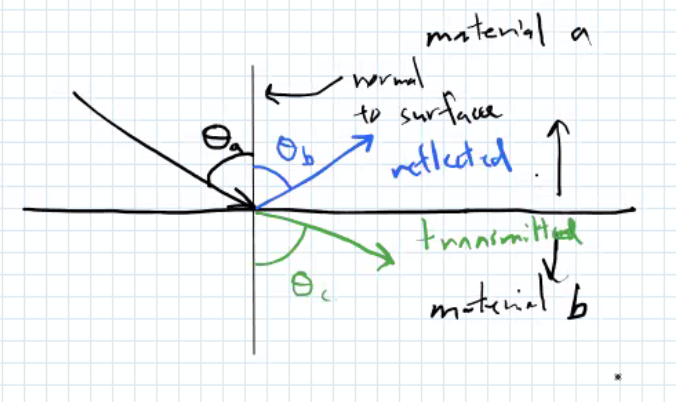
\includegraphics[width=8cm]{images/3.2.png}
\end{figure}

We observe:
\begin{enumerate}
\item Both reflected and transmitted rays are in the same plane as the incident ray and normal. 
\begin{enumerate}
\item as each other or as the original ray and normal? can we use momentum arguments with light?
\end{enumerate}
\item \underline{Law of Reflection}: $\boxed{\theta _{a} =\theta _{b}}$.
\item \underline{Snell's Law}: $\boxed{n_{a}\sin \theta _{a} =n_{c}\sin \theta _{c}}$.
\end{enumerate}

An interesting subcase of this is \underline{total internal reflection}, which is explained in "3. HW1.tex".


\
\hline
\subsection{Fermat's Principle}
\subsubsection{Paradigm Shift}
\begin{center}
\textit{``Light takes the path of least time"}
\end{center}


This might feel awkward and strange — how does light ``know" to take a certain path?



But we've encountered similar ideas in classical mechanics before in our shift from Newtonian to Lagrangian mechanics. We rearticulate mechanical systems with the \textit{Principle of Least Action}, where we consider the space of all possible configurations and observe that the system ends up choosing the route that minimizes the action.



This is relevant because we usually do physics by breaking down systems into simple parts and building back up to the whole. But when we look at the microphysical, we get to a point where we can't break things down any further. 



In this way, our ``awkward and strange" principle turns out to be more accurate, powerful, and bedrock description of reality.


\subsubsection{Deriving the Law of Reflection with Fermat's Principle}

Consider a \textit{reflection}:

\begin{figure}[htp]
    \centering
    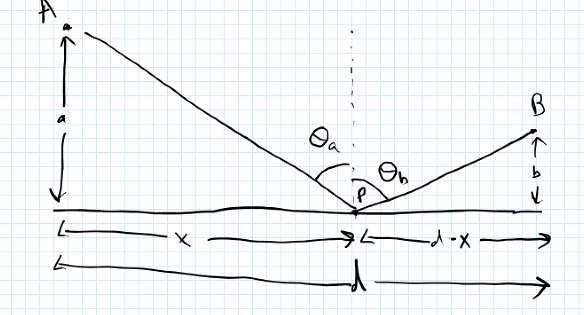
\includegraphics[width=8cm]{images/3.3.png}
\end{figure}

The distance $L$ the ray travels from $A$ to $B$ is given by
\begin{align*}
L & =\sqrt{x^{2} +a^{2}} +\sqrt{( d-x)^{2} +b^{2}} .
\end{align*}
\textbf{With the principle of least distance in mind, we minimize }$L$\textbf{ by setting its derivative equal to zero} to find:
\begin{align*}
\frac{dL}{dx} & =0\\
\frac{x}{\sqrt{x^{2} +a^{2}}} +\frac{-( d-x)}{\sqrt{( d-x)^{2} +b^{2}}} & =0\\
\frac{x}{\sqrt{x^{2} +a^{2}}} & =\frac{( d-x)}{\sqrt{( d-x)^{2} +b^{2}}} .
\end{align*}
Looking back at the diagram, we find some neat trigonometry that gives us the Law of Reflection:
\begin{align*}
\sin \theta _{a} & =\sin \theta _{b}\\
\Aboxed{\theta _{a} & =\theta _{b} .}
\end{align*}

\subsubsection{Deriving the Snell's Law with Fermat's Principle}

Consider \textit{transmission}:

% \clearpage

\begin{figure}[htp]
    \centering
    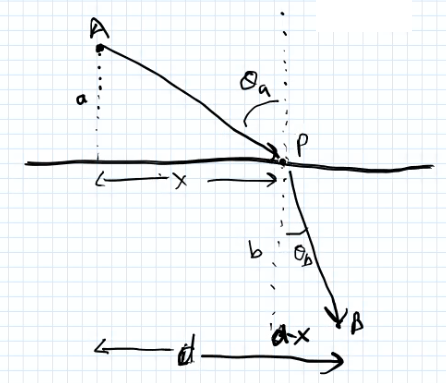
\includegraphics[width=6cm]{images/3.4.png}
\end{figure}

Before least distance and least time were equivalent. But since $v$ is no longer constant, we deal with the principle of least time. 



The time it takes to get from point A to B is:
\begin{align*}
T & =\frac{\sqrt{a^{2} +x^{2}}}{v_{a}} +\frac{\sqrt{( d-x)^{2} +b^{2}}}{v_{b}} .
\end{align*}
With a similar approach as 3.2.2 shows, we set $\tfrac{dT}{dx} =0$ and do some math/trig to find: 
\begin{align*}
\frac{\sin \theta _{a}}{v_{a}} & =\frac{\sin \theta _{b}}{v_{b}} ,
\end{align*}
and using equation 3 ($n_{x} =\tfrac{c}{v_{x}}$), we get Snell's Law:
\begin{equation*}
\boxed{n_{a}\sin \theta _{a} =n_{b}\sin \theta _{b} .}
\end{equation*}

\newpage

\hline
\section{Dispersion}
\subsection{Wave-Approach}

We observe the velocity of the ray of light change when it crosses the boundary. Since $v=\lambda f$, atleast one of those has to change. Thus, we want to understand what happens to the wavelength and frequency of a ray of light once it crosses a boundary.

\

Consider light shining directionly at a surface:

\begin{figure}[htp]
    \centering
    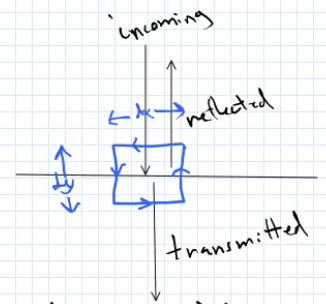
\includegraphics[width=6cm]{images/4.1.png}
\end{figure}

\textit{(Boundary condition argument:) }We're going to use Ampere's Law (Gauss's Law but with B and loops) to understand the wave constraints. 

\

The Amperian loop is drawn (CC) in blue, with some $dx$ and $dy$. The \textbf{incoming} electric field is given by:
\begin{align*}
\overrightarrow{E_{i}} & =E_{i}\cos( -k_{i} y-w_{i} t)\hat{x} ,
\end{align*}
the \textbf{reflected} electric field (perserving "handedness" of angular momentum) is given by:
\begin{equation*}
\overrightarrow{E_{r}} =E_{r}\cos( k_{r} y-w_{r} t)\left( -\hat{x}\right) ,
\end{equation*}
and the \textbf{transmitted} electric field is given by:
\begin{equation*}
\overrightarrow{E_{t}} =E_{t}\cos( -k_{t} y-w_{t} t)\left( -\hat{x}\right) ,
\end{equation*}
WLOG, we can choose $\phi =0$ because all $\vec{E}$ is in phase. 

\

Now using Ampere's law, we evaluate:
\begin{align*}
\oint \vec{E} \cdot d\vec{l} = & \ \ \ E_{i}\cos( -k_{i} y-\omega _{i} t) \cdot ( -dx)\\
 & +E_{r}\cos( k_{r} y-w_{r} t) \cdot ( dx)\\
 & +E_{t}\cos( -k_{t} y-w_{t} t) \cdot ( dx)\\
 & =\tfrac{dB}{dt} \cdot dxdy.
\end{align*}
\textit{(Note: not sure why the dot products work out like that)}

Now if we take the limit as $dy\rightarrow 0$ to simulation the boundary, we set the above equal to zero which reveals:
\begin{equation*}
E_{i}\cos( -k_{i} y-\omega _{i} t) =E_{r}\cos( k_{r} y-w_{r} t) +E_{t}\cos( -k_{t} y-w_{t} t) .
\end{equation*}
This must be true for all $t$ (?), meaning
\begin{equation*}
\omega _{i} =\omega _{r} =\omega _{t} .
\end{equation*}
\textbf{Thus, since freqency is constant, the boundary must change the wavelength.} Specifically, in the equation, we would see $k=\frac{2\pi }{\lambda }$ change. This makes sense, as IRL we observe "dispersion":

\begin{figure}[htp]
    \centering
    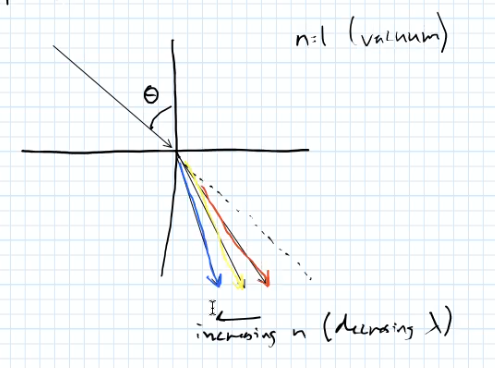
\includegraphics[width=8cm]{images/4.2.png}
\end{figure}

But this finding also lets us define ($\lambda _{0}$ and $c$ describe light in a vacuum):
\begin{align*}
n & =\frac{c}{v}\\
 & =\frac{f\lambda _{0}}{f\lambda }\\
\Rightarrow \Aboxed{\lambda  & =\frac{\lambda _{0}}{n}} \numberthis
\end{align*}
\

\hline
\subsection{Particle-Approach}

The energy of a photon is given by
\begin{equation*}
E=hf.
\end{equation*}
(Note: $h=6.6\times 10^{-34} \ J\cdot s$)

But since $c=\lambda f$, our prior results seem to indicate the light loses energy somehow. How?



\newpage

\hline
\section{Interference}

Due to superposition, waves characteristically demonstrate \underline{interference:}

\begin{figure}[htp]
    \centering
    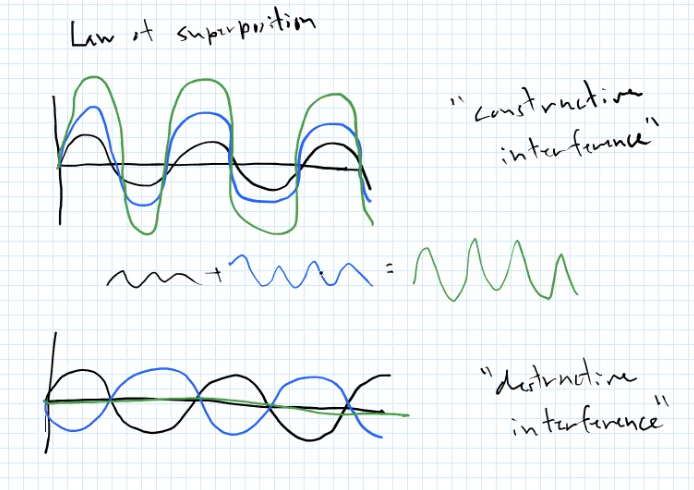
\includegraphics[width=10cm]{images/4.3.png}
\end{figure}

\

Given two sources of propogating waves $A$ and $B$, we want to find whether there's constructive or destructive interference at a certain point $P$:

\begin{figure}[htp]
    \centering
    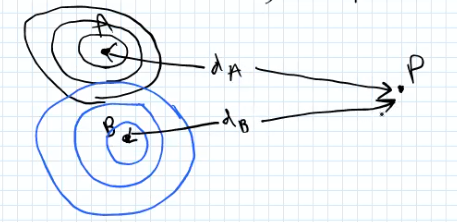
\includegraphics[width=8cm]{images/4.4.png}
\end{figure}

Let $m\in \mathbb{Z}$. Then we observe constructive interference iff
\begin{equation}
d_{A} -d_{B} =m\lambda ,
\end{equation}
and destructive interference iff
\begin{equation}
d_{A} -d_{B} =\left( m+\frac{1}{2}\right) \lambda .
\end{equation}



%%%%%%%%%%%%%%%%%%%%%%%%%%%%%%%%%%%%%%%%%%%%%%%%%%%%%%%%%%%%%%%%%%%%%%%%%%%%%%%%%
\end{document}